% Diese Zeile bitte -nicht- aendern.
\documentclass[course=erap]{aspdoc}


%notations
\usepackage{polynom}
\usepackage{amssymb}
\usepackage[utf8]{inputenc}
\usepackage{tcolorbox}
\usepackage{graphicx}
\graphicspath{ {./graphics/} }
\usepackage{xcolor}
\usepackage{listings}
\definecolor{mGray}{rgb}{0.5,0.5,0.5}
\definecolor{backgroundColour}{rgb}{0.95,0.95,0.92}
\lstdefinestyle{CStyle}{
    backgroundcolor=\color{backgroundColour},   
    commentstyle=\color{mGreen},
    keywordstyle=\color{magenta},
    numberstyle=\tiny\color{mGray},
    stringstyle=\color{mPurple},
    basicstyle=\footnotesize,
    breakatwhitespace=false,         
    breaklines=true,                 
    captionpos=b,                    
    keepspaces=true,                 
    numbers=left,                    
    numbersep=5pt,                  
    showspaces=false,                
    showstringspaces=false,
    showtabs=false,                  
    tabsize=2,
    language=C
}
\lstset{
    basicstyle=\ttfamily,
    frame=none, % Remove the frame
    language=C,
    showstringspaces=false,
    breaklines=true,
    breakatwhitespace=true,
    tabsize=4,
    numbers=left,
    numberstyle=\tiny,
    numbersep=5pt,
    keywordstyle=\color{blue},
    commentstyle=\color{green!50!black},
    stringstyle=\color{red}
}

%Graphen
\usepackage{pgfplots}
\usepackage{caption}


%%%%%%%%%%%%%%%%%%%%%%%%%%%%%%%%%
%% TODO: Ersetzen Sie in den folgenden Zeilen die entsprechenden -Texte-
%% mit den richtigen Werten.
\newcommand{\theGroup}{146} % Beispiel: 42
\newcommand{\theNumber}{A400} % Beispiel: A123
\author{Gregorius Nico Toreh \and Rafael Buala Lahagu \and Raymond King Setia}
\date{Sommersemester 2023} % Beispiel: Wintersemester 2019/20
%%%%%%%%%%%%%%%%%%%%%%%%%%%%%%%%%

% Diese Zeile bitte -nicht- aendern.
\title{Gruppe \theGroup{} -- Abgabe zu Aufgabe \theNumber}

\begin{document}
\maketitle

\section{Einleitung}

%In letzter Zeit ist die korrekte Übermittlung von Daten viel wichtiger geworden. 
    Um prüfen zu können , ob eine Nachricht korrekt und fehlerfrei übertragen wurde, kommt die sogenannte Zyklische Redundanzprüfung (englisch :  \textit{cyclic redundancy check}, daher meist \textbf{CRC}) ins Spiel. Dieser Algorithmus, der 1961 von \textit{W. Wesley Peterson} entwickelt wurde, erstellt den Prüfwert von Daten. Dadurch können Datenempfänger die Integrität der empfangenen Daten überprüfen und mögliche Fehler oder Korruptionen erkennen. Die CRC32-Berechnung basiert auf der Polynomdivision. Dabei wird der Bitstrom einer zu untersuchenden Nachricht der Länge $l$ als Polynom mit binären Koeffizienten $K_i$ dargestellt:

\[N = K_{l-1} K_{l-2} \dots K_1 K_0 \quad \hat{=} \sum_{i=0}^{l-1} K_i \cdot x^{i} =: N(x) \]

Als Dividend für die Polynomdivision wird ein sogenanntes Generatorpolynom $G(x)$ verwendet. Der Rest der Polynomdivision von
$N(x)/G(x)$ ist dann die zu berechnende Testsumme $P$. Formal gilt: 
\[(CRC32(N,G) = P(x) \equiv N(x) \quad mod \quad G(x))\]
Die Prüfsumme $P$ wird einfach nach folgender Berechnung an die erste Nachricht $N$ angehängt: $N' =(N \parallel P)$
.Nach dem Empfang der Nachricht $N'$ führt der Empfänger die identische Polynomdivision unter Verwendung des identischen $G(x)$ durch. Ist das Ergebnis 0, kann mit hoher Wahrscheinlichkeit davon ausgegangen werden, dass die Nachricht korrekt übermittelt wurde.

In diesem Projekt implementieren wir eine Funktion \textbf{CRC32} mit der Signatur:
\begin{center}
\texttt{uint32\_t CRC32(size\_t len, const char msg[len], uint32\_t generator)}
\end{center} 

Wir haben auch ein Szenario gezeigt, bei dem der CRC nicht funktioniert und die Schwachstelle des Programms aufzeigen könnte. Weitere Optimierungen wurden auch entwickelt, die die Effizienz des Prozesses verbessern können. Anschließend wird die Performanz jeder Implementierung gemessen und miteinander verglichen.



\section{Lösungsansatz}

    Es gibt verschiedene Art and Weise, wie man der CRC32 Algorithmus implementieren kann. Wir werden uns in diesem Projekt der CRC32 Algorithmus auf 3 verschiedenen Ansätzen ansehen : den algebraischen Ansatz, den bitorientierten Ansatz, und den tabelgesteuerten Ansatz. 
    
    Der algebraische Ansatz ist die mathematische Definition des CRC und besteht im Wesentlichen aus einer riesigen Polynomdivision. Dieser Ansatz enthält jedoch oft zu viel Mathematik, wenn man den Code schreiben möchte. Aus diesem Grund werden wir uns auch den bitorientierten Ansatz ansehen, bei dem die Polynomdivision in der Praxis direkt mit den Bits der Eingangsdaten durchgeführt wird.
    
    Schließlich gibt es den tabellengesteuerten Ansatz, der dieselbe Arbeit auf schnellere und effizientere Weise erledigt, weshalb dies die Art und Weise ist, wie Programme in der realen Welt das CRC tatsächlich berechnen.\cite{stigge2006reversing}



 

\subsection{Algebraischer Ansatz}
Mehr oder weniger ist das CRC gemäß der Definition eine riesige Polynomdivision.Die Eingabe, deren Typ String ist,  wird als Koeffizienten eines riesigen Polynoms interpretiert, das durch ein gegebenes CRC-Polynom, also das sogenannte Generatorpolynom $G$ dividiert wird. Der Rest dieser Division ist dann die Prüfsumme. Im Folgenden möchten wir ein Beispiel betrachten, das den CRC4-Algorithmus mit einer 7 Bit langen Eingabe veranschaulicht. Anschließend werden wir erkennen können, wie eng verwandt der algebraische Ansatz und der bitorientierte Ansatz tatsächlich sind und dass eine herkömmliche Polynomdivision für den CRC-Algorithmus nicht geeignet ist.\\
\\
\textbf{Beispiel mit CRC4 :} \\
Nachricht = 1 1 0 1 1 0 1 \\
Generatorpolynom = 1 0 1 0 1 = $x^4+x^2+1$ \\ 
Der Divisor hat 5 Bits (daher ist dies ein CRC-4-Polynom), also werden 4 Nullbits an das Eingabemuster angehängt.\\
N mit angehängten Nullen = N + 0 = 1 1 0 1 1 0 1 0 0 0 0 = $x^{10}+x^9+x^7+x^6+x^4$\\
\begin{figure}[H]
    \centering
      \begin{tcolorbox}[colback=gray!10, colframe=gray!50, arc=5pt, fontupper=\tiny, width=10cm]
        \polylongdiv{x^{10}+x^9+x^7+x^6+x^4}{x^4+x^2+1}
    \end{tcolorbox}
    \caption{normale Polynomdivision, die wir kennen}
\end{figure}
    Wie wir sehen können, enthält das Ergebnis der Polynomdivision, das die Prüfsumme für den CRC-Algorithmus darstellt, Koeffizienten, die größer als 1 und kleiner als 0 sind. Diese sind jedoch nicht mit Bits darstellbar, da Bits nur 1 darstellen können, wenn das Polynom existiert und 0, wenn es nicht existiert.

    Was wir tun können, um diese in Bits darzustellen, ist die Verwendung eines mathematischen Tricks namens endlicher Körper. Algebra ist im Grunde der Satz von Regeln, mit denen man Symbole für Operationen manipulieren kann. Zum Beispiel :
\[ \frac{x}{2} - 5 = 7 \]
Wir addieren 5 zu beiden Seiten der Gleichung \textit{(additive Eigentschaft der Gleichheit)}.
\[ \frac{x}{2} - 5 + 5 = 7 + 5\]
\[\frac{x}{2} = 12\]
Wir multiplizieren beide Seiten der Gleichung mit 2 \textit{(multiplikative Eigentschaft der Gleichheit)}.
\[\frac{x}{2} \cdot2 = 12 \cdot2\]
\[x = 24\]
    Wenn wir also nach x auflösen, wenden wir jedes Mal, wenn wir Algebra machen, eine Reihe von Regeln an.Die Zahl, die wir verwenden, wenn wir Algebra anwenden, nennt man Körper.
    
    In diesem Fall haben wir den Körper der reellen Zahlen $\mathbb{R}$ verwendet. Es gibt viele Körper in der Algebra, zum Beispiel die natürlichen Zahlen $\mathbb{N}$ und die komplexen Zahlen $\mathbb{C}$.Wir interessieren uns für endliche Körper. Wie der Name schon sagt, verwenden endliche Körper eine endliche Anzahl von Zahlen, aber die Regeln der Algebra funktionieren trotzdem gleich.
    
    Ein Körper ist im Grunde genommen eine Menge von Zahlen. Um zu definieren, wie Operationen zwischen diesen Zahlen funktionieren, müssen wir Körperaxiome einführen. Unser Körper $\mathbb{F}_2$ besteht nur 2 Zahlen: 0 und 1.Also $\mathbb{F}_2 = [0, 1]$. 
\begin{figure}[H]
    \centering
    \begin{tcolorbox}[colback=gray!10, colframe=gray!50, arc=5pt]
    \begin{tabular}{@{}ll@{\hspace{-5pt}}l@{}}
    \textbf{Assoziativität} & : $a + (b + c) = (a + b) + c$ & | $a \cdot (b \cdot c) = (a \cdot b) \cdot c $\\
    \textbf{Kommutativität} & : $a + b = b + a$ &  | $a \cdot b = b \cdot a$\\
    \textbf{Identität} & : $a + 0 = a$ & | $a \cdot 1 = a$\\
    \textbf{Additive Inverse} & : $a + (-a)= 0$ & \\
    \textbf{Multiplikative Inverse} & : $a \cdot \frac{1}{a}= 1$ & \\
    \textbf{Distributivität} & : $a \cdot (b + c)= (a \cdot b ) + (a \cdot c)$ & \\
    \end{tabular}
    \end{tcolorbox}
    \caption{Körperaxiome}
\end{figure}
Mit den oben erstellten Feldaxiomen können wir Addition, Subtraktion, Multiplikation und Division wie folgt definieren : 
\begin{figure}[H]
    \centering
    \begin{tcolorbox}[colback=gray!10, colframe=gray!50, arc=5pt, width=0.85\textwidth, fontupper=\small]
         $0 + 0 = 0$ \qquad $0 - 0 = 0$ \qquad $0 \cdot 0 = 0$ \qquad $\frac{0}{1} = 0$ \\
\\
        $0 + 1 = 1$ \qquad $0 - 1 = 1$ \qquad $0 \cdot 1 = 0$ \qquad $\frac{1}{1} = 1$ \\

        $1 + 0 = 1$ \qquad $1 - 0 = 1$ \qquad $1 \cdot 0 = 0$ \qquad $\frac{1}{0} =\infty$\\

        $1 + 1 = 0$ \qquad $1 - 1 = 0$ \qquad $1 \cdot 1 = 1$ \qquad $\frac{0}{0} =\,$\textit{undefiniert}
    \end{tcolorbox}
    \caption{neu definierte Operationen nach den Axiomen}

\end{figure}
Durch die Definition der Operationen auf diese Weise erfüllen wir alle Körperaxiome. Daher handelt es sich um einen gültigen Körper, obwohl es einige gegensätzliche Dinge gibt, die wir möglicherweise nicht erwarten.Zum Beispiel müssen wir das \textbf{additive Inverse} haben.Daher können wir sagen,dass $a + (-a) = 0$ ist. In unserem Körper ist das additive Inverse einer Zahl die Zahl selbst. Zum Beispiel ist das additive Inverse von $1$ ebenfalls $1$, und auch $1 + 1 = 0$. Als nächstes betrachten wir ein Beispiel, in dem die Axiome angewendet wurden. \\
\begin{figure}[H]
    \centering
    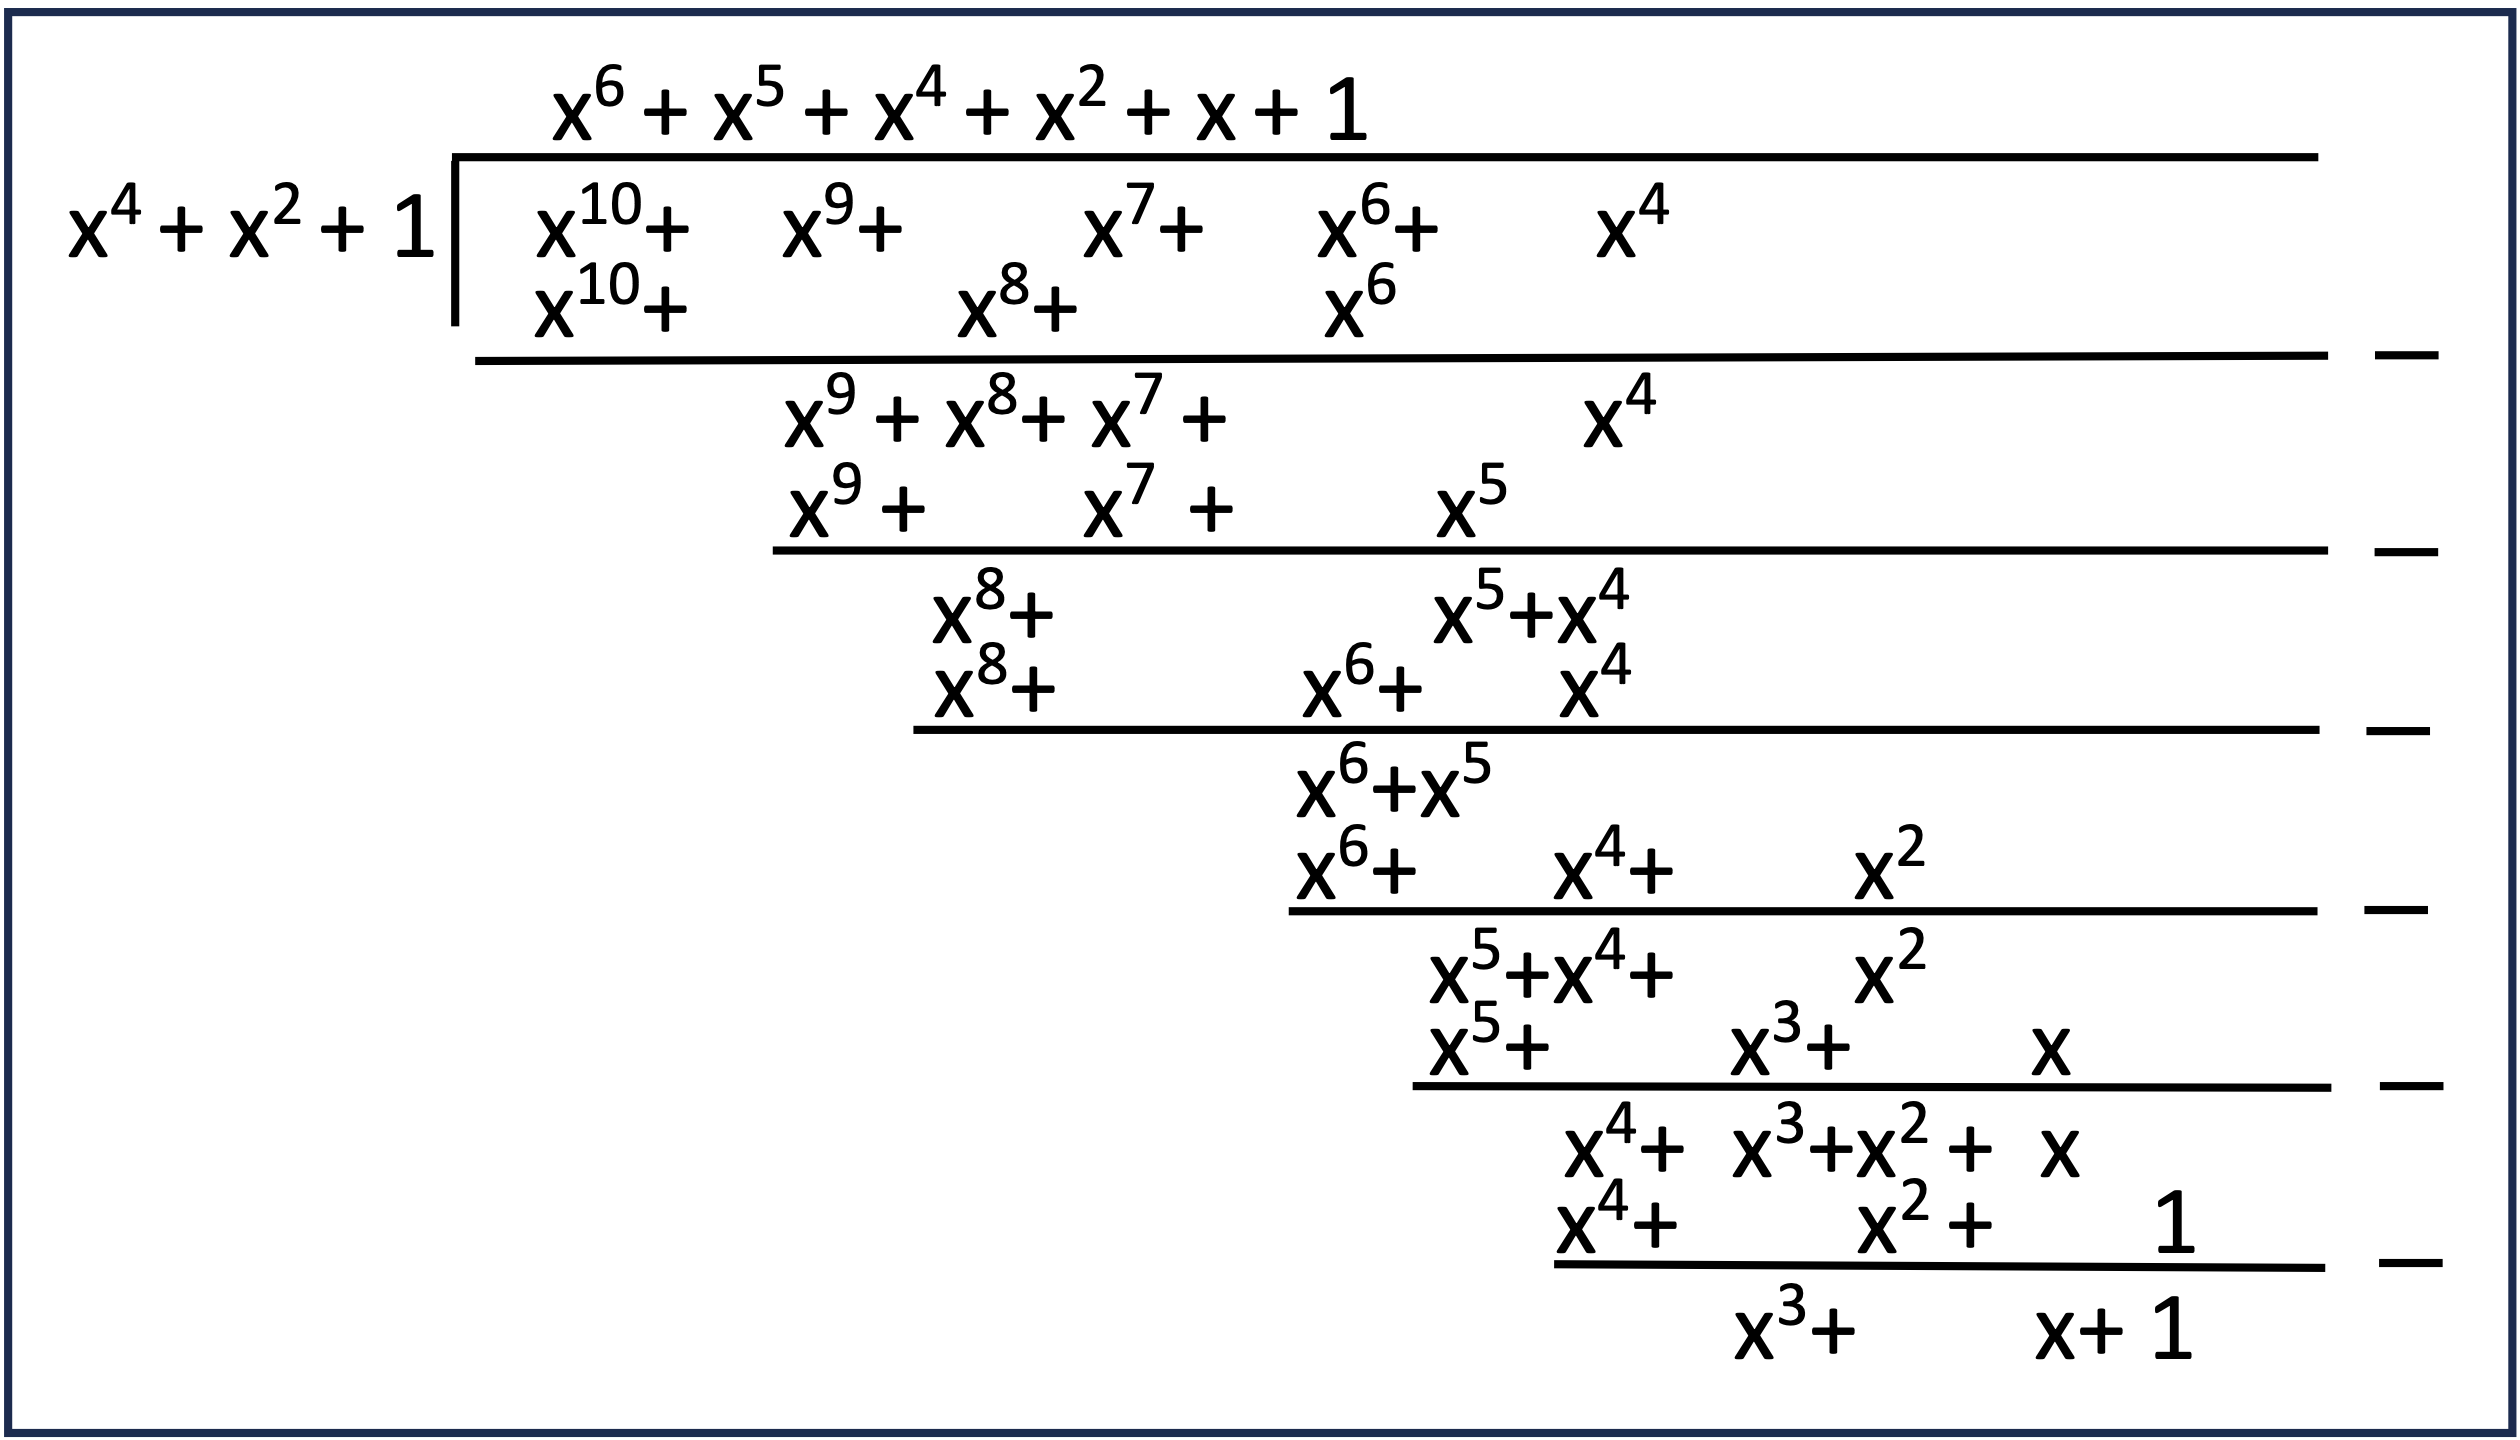
\includegraphics[width=8cm, height=5cm]{polynomialdivision}
    \caption{Polynomdivision mit vordefinierten Axiomen}
    \label{fig:enter-label}
\end{figure} 
Der Rest der Polynomdivision $x^3+x+1$  stellt die Prüfsumme $1 0 1 1$ für den CRC-Algorithmus dar. Jetzt kann man sehen, dass es keine Koeffizienten gibt, die größer als $1$ und kleiner als $0$ sind, und kann daraus schließen, dass dieses Polynom nun mit Bits darstellbar ist.

\subsection{Bitorientierter Ansatz}
Nun wird die dort oben definierten Operationen betrachtet, die auf den Körperaxiomen beruhen. Das Ergebnis der möglichen Eingabekombinationen für Addition und Subtraktion stellt tatsächlich die Wahrheitstabellen-XOR-Operation dar.
\begin{figure}[H]
    \centering
    \begin{tabular}{|c|c|c|}
        \hline
        $A$ & $B$ & $A \oplus B$ \\
        \hline
        0 & 0 & 0 \\
        0 & 1 & 1 \\
        1 & 0 & 1 \\
        1 & 1 & 0 \\
        \hline
    \end{tabular}
    \caption{Wahrheitstabelle der XOR-Operation}
\end{figure}
Wir haben die Funktion
\begin{center}
\texttt{uint32\_t CRC32\_V2(size\_t len, const char msg[len], uint32\_t generator)}
\end{center} 
mit der Programmiersprache C implementiert. Anschließend können wir sehen, wie sich die XOR-Operationen verhalten und wie wir sie für die CRC-Berechnung ausnutzen können.
\begin{lstlisting}[style=CStyle]
uint32_t CRC32_V2(size_t len, const char msg[len], uint32_t generator) {
    uint32_t result = 0; 
    for (size_t i = 0; i < len; i++) { 
        result ^= (uint32_t)(msg[i] << 24);
        for (size_t j = 0; j < 8; j++) { 
            if ((result & 0x80000000)) {  
                result = (uint32_t)((result<<1)^generator);
            } else{
                result <<=1;   
            }
        }
    }
    return result; 
}
\end{lstlisting}
    Die Methode \textbf{CRC32\_V2} nimmt die Eingabe in Form eines Nachrichtenarrays \textbf{msg} an und verarbeitet sie byteweise. Die Berechnung der CRC-Prüfsumme erfolgt jedoch bitweise innerhalb jedes Bytes. Dabei wird das Ergebnis schrittweise aktualisiert, indem die XOR-Operation auf die entsprechenden Bits angewendet wird. Am Ende wird die vollständige CRC-Prüfsumme zurückgegeben.
\subsection{Ansatz mit Umsetzungstabelle}
Die Art und Weise, wie dieser tabellengesteuerte Ansatz funktioniert, unterscheidet sich nicht wesentlich vom bitorientierten Ansatz. Aber anstatt eine XOR-Operation an der Bitfolge durchzuführen, erstellen und berechnen wir zunächst eine Umsetzungstabelle \textit{(englisch : Lookup-Table)} mit dem eingegebenen Generatorpolynom. 

Die Größe der Tabelle beträgt 256, da die Größe eines Characters \textit{(char)} 8 Bit beträgt und es daher 256 mögliche Eingaben für das Character gibt. Nun werfen wir einen Blick auf die Methode, mit der man die Umsetzungstabelle erstellen kann.\\ 
\begin{lstlisting}[style=CStyle]
 void crc32TableFillSIMD(uint32_t* table, uint32_t generator) {
    __m128i genpoll = _mm_set1_epi32(generator);
    for (int i = 0; i < 256; i += 4) {
        __m128i res = _mm_slli_epi32(_mm_set_epi32(i+3, i+2, i+1, i), 24);
        for (uint8_t j = 8; j > 0; j--) {
            __m128i msb = _mm_srai_epi32(res, 31);
            res = _mm_slli_epi32(res, 1);

            __m128i r = _mm_and_si128(msb, genpoll);
            res = _mm_xor_si128(res, r); 
        }
        _mm_storeu_si128((__m128i*)&table[i], res); 
    }
}
\end{lstlisting}
Der Code verwendet SIMD-Anweisungen, um eine CRC32-Lookup-Tabelle mit dem gegebenen Generatorpolynom zu füllen. Die Funktion \textbf{crc32TableFillSIMD} nimmt einen Zeiger auf die Lookup-Tabelle \textbf{table} und das Generatorpolynom \textbf{generator} entgegen.

Der Code verwendet SIMD-Register, um mehrere Operationen parallel auszuführen und die Effizienz zu verbessern.Die äußere Schleife iteriert über die Indizes der Lookup-Tabelle. In jedem Schleifendurchlauf werden vier Einträge gleichzeitig berechnet.

Die innere Schleife führt acht Iterationen aus, um die CRC-Berechnung für jeden Index zu vollziehen. Am Ende wird das Ergebnis aus den SIMD-Registern in die Lookup-Tabelle geschrieben.

Man kann dann den Wert (0x00 -0xFF) aus der Lookup-Tabelle abrufen, anstatt XOR-Operationen durchzuführen. Aus diesem Grund müssen wir denselben Wert nicht immer wieder neu berechnen, wenn die Eingabe viele gleiche Werte enthält.
% TODO: Je nach Aufgabenstellung einen der Begriffe wählen
\section{Korrektheit}
Die Korrektheit des CRC32-Algorithmus ist entscheidend für die Gewährleistung der Datenintegrität. Dabei stehen zwei Hauptaspekte im Fokus: die deterministische Erzeugung des Prüfwerts und die zuverlässige Erkennung von Fehlern. Ein guter CRC32-Algorithmus erzeugt für eine gegebene Datenfolge immer denselben Prüfwert und hat eine hohe Wahrscheinlichkeit, fehlerhafte Daten zu identifizieren, während die Fehlalarmrate für korrekte Daten gering sein sollte.
\subsection{Generatorpolynom}
Beginnen wir damit, zu untersuchen, wie man ein geeignetes Generatorpolynom $G$ auswählen kann, um die Wahrscheinlichkeit einer zuverlässigen Fehlererkennung zu maximieren\cite{williams1993painless}. Um dies zu veranschaulichen, betrachten wir ein Beispiel.\\
Der Empfänger bekommt ein Generatorpolynom $G = 1\:1\:0\:1\:0\:1$ und eine Nachricht $N'$.\\
\\
Fallunterscheidung : \\
\textbf{Fall 1 :} $N' \quad\;\;\;\:= 1\:\textbf{1}\:0\:1\:1\:0\:0\:1\:0\:1 = x^9+x^8+x^6+x^5+x^2+1\:mod\:G = 0$\\
\textbf{Fall 2 :} $N'_{Fehler} = 1\:\textbf{0}\:0\:1\:1\:0\:0\:1\:0\:1 = x^9+\qquad \,\,x^6+x^5+x^2+1\:mod\:G = x^4+x^2+x$\\
\textbf{Fall 3 :} $N'_{Fehler} = 1\:\textbf{0}\:\textbf{1}\:\textbf{0}\:1\:0\:0\:1\:\textbf{1}\:1 = x^9+\;\;x^7+x^5+x^2+x+1\:mod\:G = 0$\\
\\
Im ersten Fall handelt es sich um die richtige Nachricht, im zweiten und dritten Fall nicht.Die Nachricht im dritten Fall unterscheiden sich an 4 Stellen der Bitfolge. Das Generatorpolynom $G$ teilt aber das Polynom $x^9+x^7+x^5+x^2+x+1$, deshalb ist die Prüfsumme wieder gleich 0. Der Empfänger kann nicht feststellen, dass ein Fehler stattgefunden hat, weil er bei dem Prüfsumme = 0 davon ausgehen muss, dass wohl alles in Ordnung ist. Das Ziel dieses Verfahrens ist es auch, den 3. Fall zu vermeiden. \\

Wir zerlegen jetzt die falsche Nachricht $N'_{Fehler}$ im dritten Fall in zwei Teilen. Einmal das richtige Polynom $N'$ was eigentlich versendet wurde, und die Bitfolge $e$, an deren Stellen es Fehler gegeben hat.
\begin{center}
$N'_{Fehler} = 1\:\textbf{0}\:\textbf{1}\:\textbf{0}\:1\:0\:0\:1\:\textbf{1}\:1$ \\
$N' \quad\;\;\;\:= 1\:\textbf{1}\:0\:1\:1\:0\:0\:1\:0\:1$ \\
$e \quad\;\;\;\;\;\;\,= 0\:\textbf{1}\:\textbf{1}\:\textbf{1}\:0\:0\:0\:0\:\textbf{1}\:0$\\
\end{center}
Wenn man eine bitweise XOR Operation auf $N'$ und $e$ anwendet, dan erhält man wieder $N'_{Fehler}$. Wir wissen, dass $G$ ein Teiler von $N'_{Fehler}$ ist, also $G\,|\,N'_{Fehler}$. Aus $N'_{Fehler} = N' + e$ folgt, dass $G\,|\,(N' + e)$. Wir wissen auch, dass $G\,|\,N'$. Daraus folgt, dass $G\,|\,e$.Das ist die Sache, die wir vermeiden möchten. Das heißt, wir können jetzt Fehlerpolynomen aussuchen, die wir erkennen möchten, und die dürfen alle nicht Vielfache von $G$ sein. Das ist das was man finden muss, wenn man ein gutes $G$ haben möchte. \\

Nun betrachten wir die erste Anforderung an das Generatorpolynom $G$ genauer. Wenn $pq$ das Produkt von 2 Polynomen $p$ und $q$, dann kann $pq$ nur dann ein Monom $x^k$ sein, wenn $p$ und $q$ beide Monome sind. Anders ausgedrückt, wenn unser Generatorpolynom $G$ selbst kein Monom ist, dann kann $G$ auch das Fehlerpolynom $e$ nicht teilen, wenn $e$ ein Monom ist. \\

Die zweite Art von Fehler, die man gerne erkennen möchte, ist die sogenannten Bündelfehler. Dabei geht es darum, dass eine ganze Reihe von Fehlern in einem räumlich begrenzten Bereich auftreten. Hier nehmen wir einen Bündelfehler der Länge 4. Also $e = \underline{\textbf{1}\:0\:\textbf{1}\:\textbf{1}}\:0\:0 = x^5+x^3+x^2 = (x^3+x+1)\cdot{x^2}$.Das muss aber nicht heißen, dass alle 4 Stellen fehler sein müssen. Die faktoren $(x^3+x+1)$ und ${x^2}$ sind teilerfremd,das heißt, wenn $G\,|\,e$ ist, dann muss $G\,|\,(x^3+x+1)$, weil wir oben schon ausgeschlossen, dass $G$ kein Monom ist. Das geht aber nur, wenn der Grad von $G$ höchstens 3 ist. Also die zweite Forderung die wir formulieren können ist, dass $G$ möglichst hohen Grad haben soll, damit dann Bündelfehler erkannt werden können, die nicht breiter als der Grad von G ist. Aber je höher der Grad des Generatorpolynoms ist, desto höher ist auch natürlich die Redundanz, da man mehr Stellen hinter der Nachricht als Prüfbits hängen muss.\\

Die dritte wünschenswerte Eigenschaft des Generatorpolynoms, die man gerne hätte,ist, dass $G$ möglichst viele Polynome der Form $x^k+1$ nicht teilen,damit Fehler, die aus 2 Bits bestehen, deren Abstand nicht zu größ ist, erkannt werden können. Zum Beispiel wenn das Fehlerpolynom $e = 1\:0\:0\:0\:0\:0\:0\:0\:1$ ist.Ein Beispiel aus der Praxis für das Generatorpolynom, das häufig Im Ethernet Protokoll (IEEE802.3) eingesetzt wird, ist das Polynom $G =  x^{32} + x^{26} + x^{23} + x^{22} + x^{16} + x^{12} + x^{11} + x^{10} + x^8 + x^7 + x^5 + x^4 + x^2 + x + 1$.\\

\subsection{Testing}
Wir haben eine Methode geschrieben
\begin{center}
    \texttt{void test(size\_t len, const char msg[len], uint32\_t generator, int imp)} \\
\end{center}
,um zu testen, ob die CRC32-Methoden wie erwartet ordnungsgemäß funktionieren.Das \textbf{int imp} ermöglicht es dem Benutzer, auszuwählen, welche Implementierung des CRC32-Algorithmus er testen möchte, da wir den Algorithmus auf verschiedene Arten implementiert haben.

    Zuerst suchen wir nach der Prüfsumme, die durch die gegebene Nachricht und das Generatorpolynom generiert wird. Anschließend hängen wir die Prüfsumme an die Nachricht $N$ an, wodurch eine neue Nachricht $N'$ entsteht. Anschließend führen wir die CRC32-Operation durch, indem wir zunächst $G$ an $N'$ anhängen. 
    
    Wenn das Ergebnis 0 ist, liegt beim Versenden der Nachricht möglicherweise kein Fehler oder keine Datenbeschädigung vor. Das Ergebnis dieser Methode sollte jedoch immer 0 sein, da wir die Nachricht eigentlich nirgendwohin versenden und es beim Versenden keine Fehler geben sollte.

\section{Performanzanalyse}
In unserem Rahmenprogramm wurden insgesamt drei Implementierungen V0, V1, und V2 implementiert. Die naive Implementierung (V2) verwendet die standardmäßige Bitweise Operation ohne Optimierung. Die zweite Vergleichsimplementierung (V1) verwendet eine Lookup-Tabelle,  mit vorberechneten Byte Werten für eine schnellere Laufzeit. Und die Hauptimplementierung (V0) verwendet Lookup-Table und SIMD als Optimierung. 

    Alle Tests werden auf einem System mit Intel I5-10300H, 2.50GHz, und mit 1 x 16GB DDR4 RAM unter 64 Bit Ubuntu 22.04.2 ausgeführt. Der Code ist mit GCC 11.3.0 mit der Option -O2 kompiliert.

    Die Effizienz einer Implementierung kann anhand der Leistung im Vergleich zur Rechengeschwindigkeit bewertet werden. Durch den Vergleich der Laufzeit verschiedener Implementierungen mit ähnlichen Eingaben können wir deren Effizienz vergleichen.

    Um die Performanz zu analysieren, haben wir zwei verschiedene Szenarien getestet: größere und kleinere Eingaben. Bei den  kleineren Eingaben haben wir Intervalle von 50 Bytes versucht, während wir bei den größeren Eingaben Intervalle von 1000 Bytes verwendet haben. Für die erste Grafik wird der Code 2,000,000 mal ausgeführt, und für die zweite 200,000 mal.
\begin{figure}[H]
    \centering
    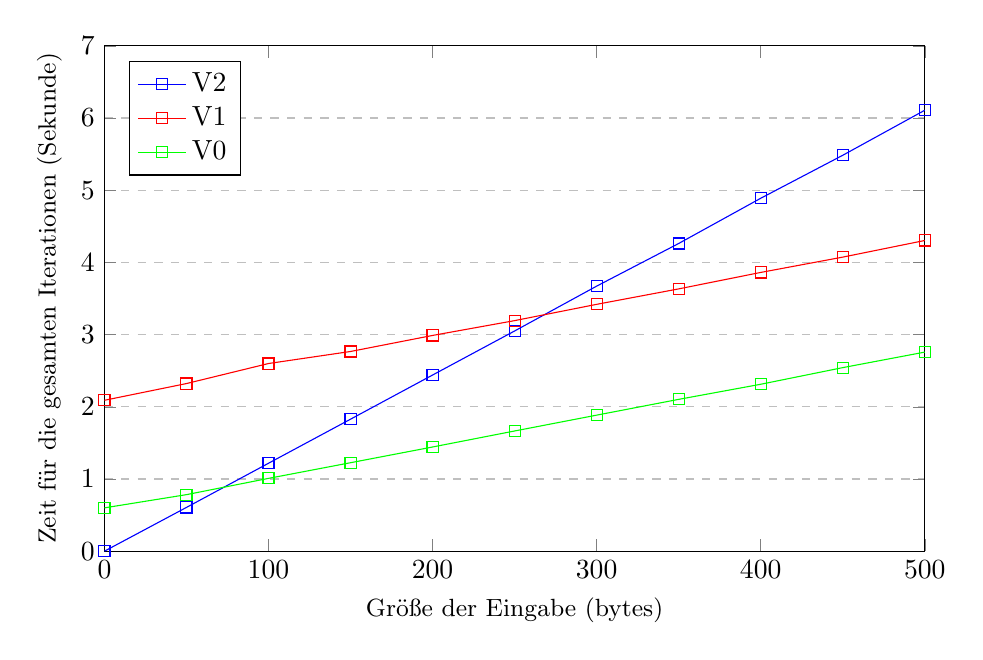
\begin{tikzpicture}
    \begin{axis}[
    width=12cm,
    height=8cm,
    xlabel={\small Größe der Eingabe (bytes)},
    ylabel={\small Zeit für die gesamten Iterationen (Sekunde)},
    xmin=0, xmax=500,
    ymin=0, ymax=7,
    xtick={0,100,200,300,400,500},
    ytick={0,1,2,3,4,5,6,7},
    legend pos=north west,
    ymajorgrids=true,
    grid style=dashed,
    ]

    \addplot[
    color=blue,
    mark=square,
    ]
    coordinates {
    (0,0)(50, 0.606116)(100, 1.217828)(150, 1.828315)(200, 2.439826)(250, 3.050103)(300, 3.671205)(350, 4.261886)(400, 4.888256)(450, 5.483677)(500, 6.107593)
    };
    \legend{V2}

    \addplot[
    color=red,
    mark=square,
    ]
    coordinates {
    (0,2.09)(50, 2.321794)(100, 2.599360)(150, 2.766103)(200, 2.988302)(250, 3.193425)(300, 3.419062)(350, 3.633025)(400, 3.861017)(450, 4.073092)(500, 4.303616)
    };
    

    \addplot[
    color=green,
    mark=square,
    ]
    coordinates {
    (0, 0.6)(50, 0.783034)(100, 1.008468)(150, 1.225360)(200, 1.443039)(250, 1.664911)(300, 1.884248)(350, 2.102949)(400, 2.312015)(450, 2.542464)(500, 2.757462)
    };
    \legend{V2, V1, V0}
    \end{axis}
    \end{tikzpicture}
    \captionsetup{font=small}
    \caption{Vergleich zwischen 3 Implementierungen von CRC32 mit 2.000.000 Iterationen}
\end{figure}

\begin{figure}[H]
    \centering
    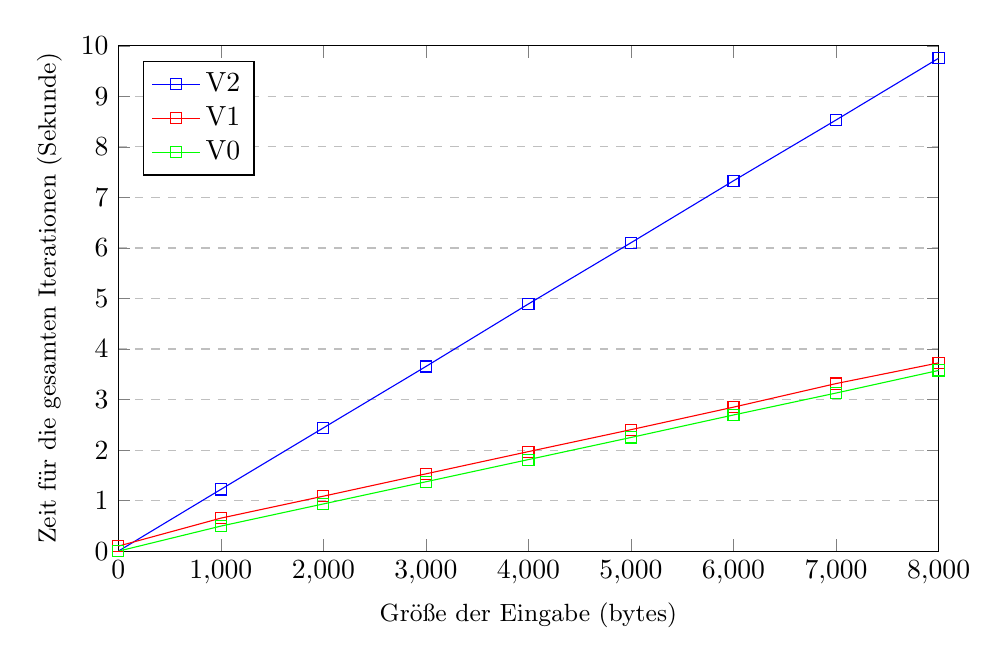
\begin{tikzpicture}
    \begin{axis}[
    width=12cm,
    height=8cm,
    xlabel={\small Größe der Eingabe (bytes)},
    ylabel={\small Zeit für die gesamten Iterationen (Sekunde)},
    xmin=0, xmax=8000,
    ymin=0, ymax=10,
    xtick={0,1000,2000,3000,4000,5000,6000,7000,8000},
    ytick={0,1,2,3,4,5,6,7,8,9,10},
    legend pos=north west,
    ymajorgrids=true,
    grid style=dashed,
    ]

    \addplot[
    color=blue,
    mark=square,
    ]
    coordinates {
    (0,0)(1000, 1.222272)(2000, 2.439483)(3000, 3.654452)(4000, 4.892223)(5000, 6.103043)(6000, 7.329283)(7000, 8.531679)(8000, 9.753619)
    };

    \addplot[
    color=red,
    mark=square,
    ]
    coordinates {
    (0,0.1)(1000, 0.653781)(2000, 1.088529)(3000, 1.530467)(4000, 1.970700)(5000, 2.404646)(6000, 2.850261)(7000, 3.316679)(8000, 3.725965)
    };

    \addplot[
    color=green,
    mark=square,
    ]
    coordinates {
    (0,0)(1000, 0.496213)(2000, 0.935169)(3000, 1.373675)(4000, 1.812705)(5000, 2.250217)(6000, 2.695594)(7000, 3.129431)(8000, 3.576482)
    };


    \legend{V2, V1, V0}

    \end{axis}
    \end{tikzpicture}
    \captionsetup{font=small}
    \caption{Vergleich zwischen 3 Implementierungen von CRC32 mit 200.000 Iterationen}
\end{figure}
    Auf der einen Seite kann man laut der ersten Grafik  deutlich sehen, dass alle drei Implementierungen stetig gestiegen sind. Bei 500 bytes Eingabe braucht V0 die geringste Zeit, nämlich fast 3 Sekunden. Das ist 2 mal schneller im Vergleich zu V2, die für gleiche Eingabe knapp 6 Sekunden braucht. Auffällig ist es, dass V0 am Anfang des Diagramms schneller ist als die Anderen. Dies könnte passieren, weil das Erstellen einer Tabelle ein Overhead ist. Das Füllen der Tabelle erzwingt zusätzlichen Speicherplatz und Zeit. Die Tabelle wird dadurch 256 Zahlen haben, von denen die meisten unnötig für kleinere Eingaben sind. V0 erfordert auch viele Speicherzugriffe, welche bei kleinen Eingaben erheblich sein können und sich auf die Leistung schlecht auswirken.

    Auf der anderen Seite ist V0, das eine Lookup-Tabelle und SIMD verwendet, etwa 0,2 Sekunden schneller als V1. Allerdings ist der Unterschied nicht so signifikant, und das aus mehreren Gründen. Einer davon ist, dass die Berechnung jedes Bytes voneinander abhängig ist und daher nicht parallel ausgeführt werden kann. Aus diesem Grund können wir SIMD nur in einem kleinen Teil des Codes verwenden und nämlich zur Berechnung der Lookup-Tabelle.

    Anhand des vorliegenden Graphen lässt sich deutlich erkennen, dass V2 oder die Naive-Implementierung wesentlich langsamer ist als V0 und V1. Dieser Geschwindigkeitsunterschied resultiert daraus, dass V2 wiederholt viele Bytes mit denselben Werten berechnet, während V0 und V1 alle Werte (0x00 - 0xFF) lediglich einmal in der Lookup-Table berechnen. Demzufolge erfordert V2 eine deutlich längere Laufzeit im Vergleich zu den anderen Implementierungen. Nach einer detaillierten Untersuchung des Graphen sind wir zu dem Schluss gekommen, dass unsere Hauptimplementierung mit Lookup-Table und SIMD die optimale Wahl für die Hauptimplementierung darstellt.

\section{Zusammenfassung und Ausblick}

    Die Ausarbeitung präsentiert drei verschiedene Implementierungen des CRC32 Algorithmus: den algebraischen Ansatz, den bitorientierten Ansatz und den tabellengesteuerten Ansatz. Der algebraische Ansatz basiert auf der mathematischen Definition des CRC und führt eine Polynomdivision durch. Der bitorientierte Ansatz führt die Polynomdivision direkt mit den Bits der Eingangsdaten durch, während der tabellengesteuerte Ansatz eine Lookup-Tabelle verwendet, um die teuren XOR-Operationen zu vermeiden.

    Es wurden auch wichtige Aspekte bei der Wahl eines geeigneten Generatorpolynoms für den CRC32-Algorithmus diskutiert. Ein gutes Generatorpolynom sollte eine hohe Wahrscheinlichkeit haben, Fehler zu erkennen, und keine Polynome der Form $x^k+1$ teilen können, um Bündelfehler zu erkennen.Die Korrektheit des CRC32-Algorithmus wird ebenfalls betrachtet, wobei die deterministische Erzeugung des Prüfwerts und die zuverlässige Erkennung von Fehlern im Fokus stehen.

    Abschließend werden Performanzanalysen der Implementierungen durchgeführt. Dabei werden verschiedene Szenarien mit unterschiedlichen Eingabegrößen getestet. Die Implementierung mit der Lookup-Tabelle und SIMD-Optimierung zeigt die beste Performanz und ist effizienter als die anderen Implementierungen.\\

    Zusammenfassend lässt sich sagen, dass der CRC32-Algorithmus recht schnell und zuverlässig ist, um zu überprüfen, ob beim Senden einer Nachricht ein Fehler aufgetreten ist. Aus diesem Grund wird dieser Algorithmus bis heute beispielsweise im Ethernet-Protokoll verwendet.

    Andere Ansätze zur Optimierung des CRC32 Algorithmus können untersucht werden,um die Geschwindigkeit und die Fähigkeit zur Fehlererkennung des Programms zu verbessern.

% TODO: Fuegen Sie Ihre Quellen der Datei Ausarbeitung.bib hinzu
% Referenzieren Sie diese dann mit \cite{}.
%Beispiel: CR2 ist ein Register der x86-Architektur~\cite{intel2017man}.


\bibliographystyle{plain}
\bibliography{Ausarbeitung}{}

\end{document}